% !TeX spellcheck = it_IT
Questo capitolo descrive le tecnologie utilizzate per lo sviluppo di un'applicazione in realtà virtuale e connessa alla rete per i Samsung GearVR.\\

\section{Unity}
\begin{wrapfigure}{rH}{0.35\textwidth} %this figure will be at the right
	\centering
	
\includegraphics[width=0.15\textwidth]{figure/UnityLogo}
\end{wrapfigure}
Unity è un motore grafico multipiattaforma sviluppato da Unity Technologies per la creazione di videogiochi (3D/2D) o di altri contenuti interattivi, quali visualizzazioni architettoniche o animazioni 3D in tempo reale.\cite{UnityDesc}
La sua ampia lista di piattaforme supportate \cite{UnityPlat} e i bassi requisiti di sistema necessari per l'uso \cite{UnityReq} lo hanno reso uno dei motori grafici più utilizzati dagli sviluppatori. L'ultima versione rilasciata è 'Unity 2017.2'. \\
A differenza di altri software, Unity permette l'utilizzo di diversi linguaggi di programmazione supportando:
\begin{itemize}
	\item C\#
	\item Javascript
	\item Boo
\end{itemize}
Nel caso di questo progetto è stato utilizzato il linguaggio C\# ed ogni porzione di codice farà riferimento ad esso.
Possono essere combinate all'interno dello stesso progetto, benché non sia buona norma. \\
Unity adotta due tipi di sotto iscrizoni per ottenere una licenza: \textit{free} e \textit{Pro}. La versione free, come si deduce dal nome, è gratuita perché pensata per un uso personale, mentre quella Pro è obbligatoria se l'organizzazione che la utilizza ha degli introiti superiori a 100.000 dollari.
Sino alla versione "Unity 4", la licenza free imponeva grosse limitazioni sullo sviluppo delle applicazioni, ma dalla versione "Unity 5" non è più così, lasciando nella licenza Pro poche funzioni esclusive, come strumenti di profilazione o di condivisione del progetto all'interno del team di sviluppo.  

\begin{figure}[t]
	\centering
	\begin{minipage}[b]{0.49\textwidth}
		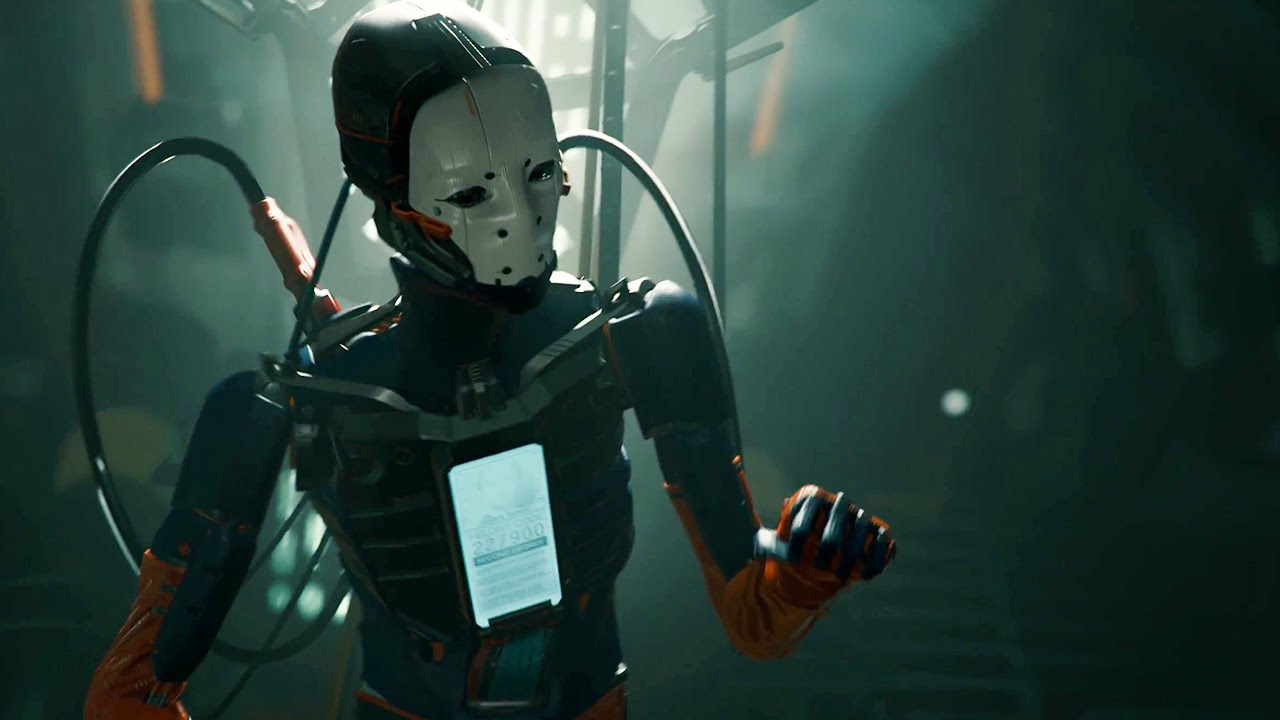
\includegraphics[width=\textwidth]{figure/Adam}
		{\footnotesize \centerline{(a)} \par}
	\end{minipage}
	\hfill
	\begin{minipage}[b]{0.49\textwidth}
		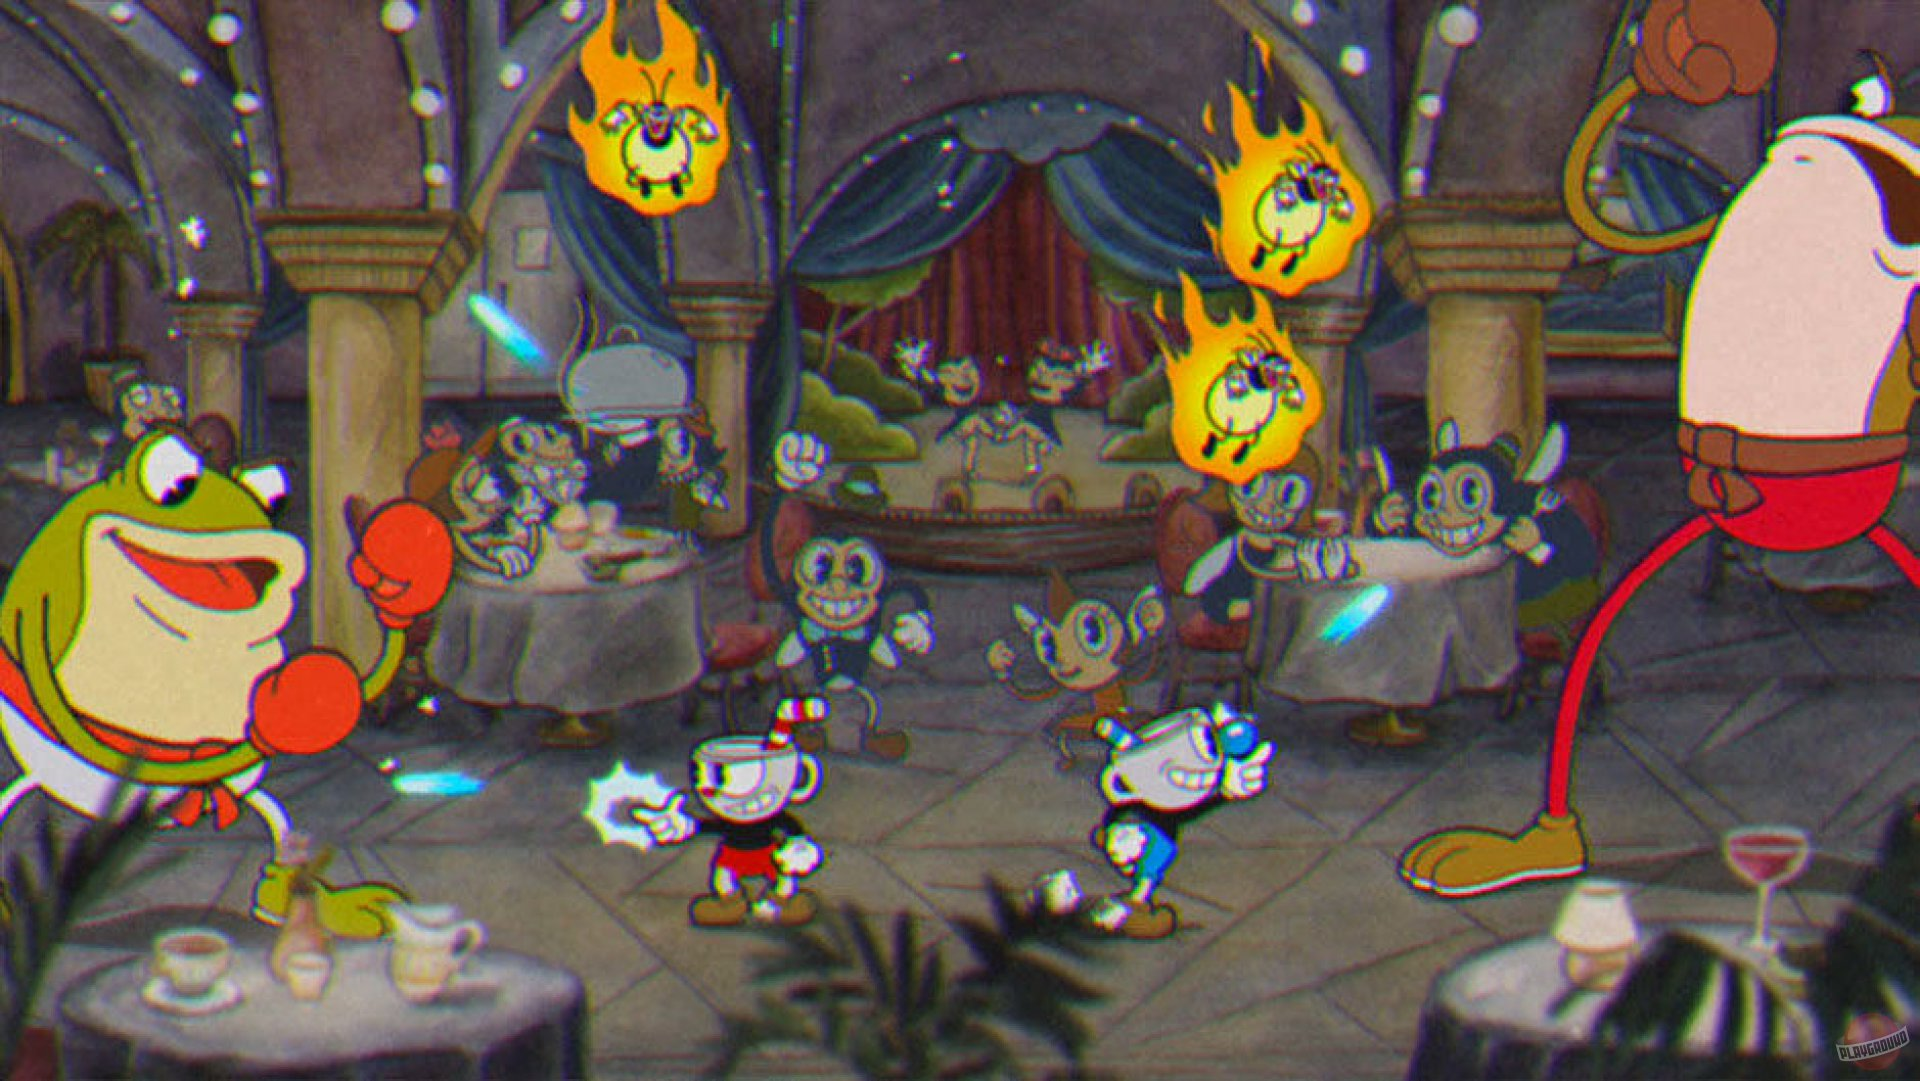
\includegraphics[width=\textwidth]{figure/Cuphead}
		{\footnotesize \centerline{(b)} \par}
	\end{minipage}
	\caption{Esempi di due giochi creati con Unity: "Adam" (3D) \cite{UnityAdam} (a) e "Cuphead" in 2D \cite{Cuphead} (b).}
\end{figure}

\newpage
Unity è stato utilizzato durante questo tirocinio poiché è risultato ottimale alla luce dei fattori chiave, considerati in termini di tempo e qualità, come mostrato nella figura sottostante.
\begin{figure}[H]
	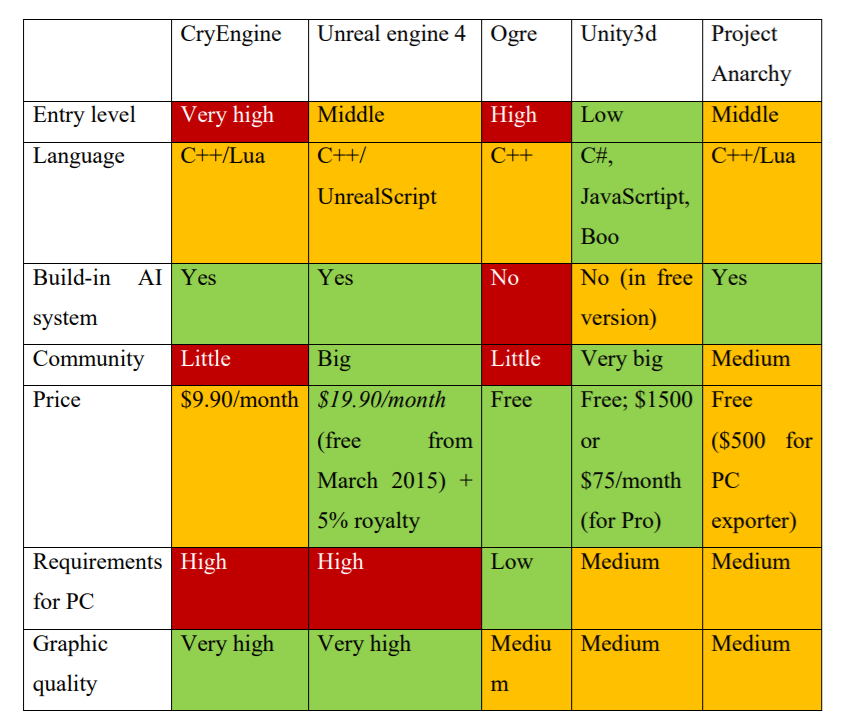
\includegraphics[width=0.85\textwidth]{figure/EngineComp}
	\centering
	\vspace{0.3cm}
\caption{Gli aspetti negativi sono colorati in rosso mentre quelli positivi sono colorati di verde. Il colore giallo viene usato per evidenziare funzioni accettabili ma che richiedono un maggiore investimento monetario o di tempo. \cite{ThesisUnity}}
\end{figure}

\newpage

\subsection{L'Editor di Unity}
Questo sottocapitolo fornisce le informazioni che concernono l'editor. Le principali sono sei \cite{UnityEditor}: 
\begin{flushleft}
	\underline{\textit{Il progetto}:}
	In questa finestra è possibile gestire e accedere alle risorse del progetto. Il pannello a sinistra mostra la struttura delle cartelle, mentre nel pannello di destra vengono mostrate le risorse interne alla cartella selezionata. Da notare come la radice della struttura sia una cartella particolare, auto generata con l'inizializzazione del progetto e denominata "Assets". Grazie alla toolbar situata in alto si possono cercare elementi all'interno del progetto.
\end{flushleft}

\begin{figure}[H]
	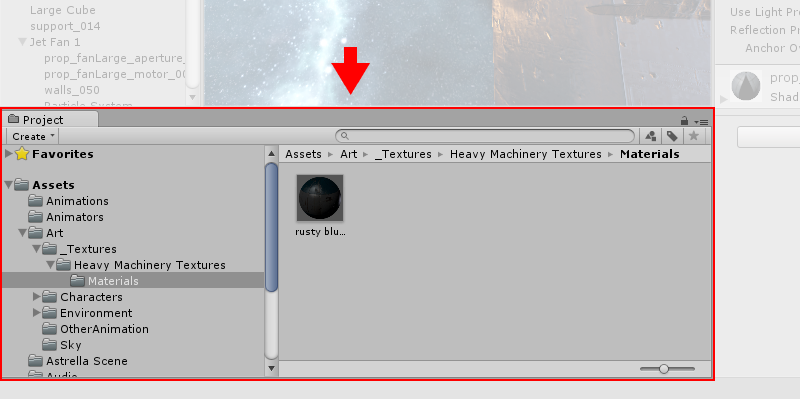
\includegraphics[width=0.55\textwidth]{figure/Project}
	\centering
	\caption{La finestra di progetto.}
\end{figure}

\begin{flushleft}
	\underline{\textit{La scena}:}
	La finestra di scena ("Scene View") fornisce una vista interattiva sul mondo virtuale che si sta creando. Da qui si possono posizionare, ruotare, scalare elementi come modelli 3D, camere, luci, e altri tipi di \textit{GameObjects} che analizzeremo più avanti.
\end{flushleft}

\begin{figure}[H]
	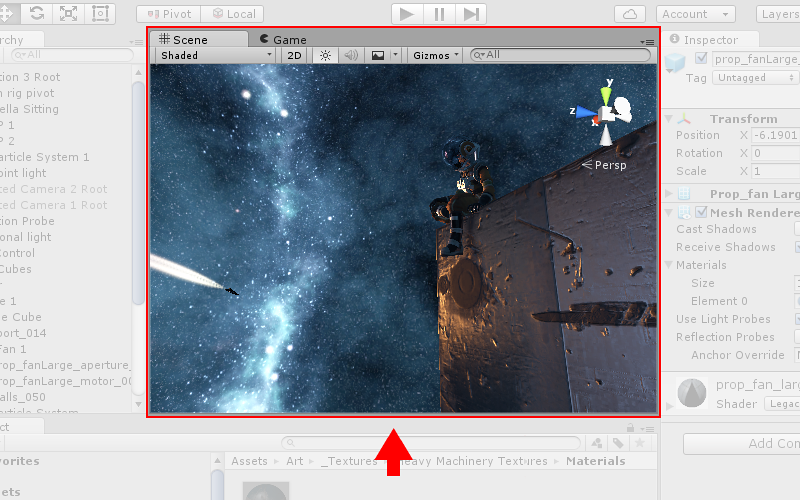
\includegraphics[width=0.45\textwidth]{figure/Scene}
	\centering
	\caption{La finestra contenente la scena.}
\end{figure}


\begin{flushleft}
	\underline{\textit{L'organigramma}:}
	Questo pannello contiene una lista di tutti gli elementi presenti nella scena corrente. Di default gli oggetti sono in ordine di inserimento, ma possono essere riordinati manualmente. Quando si annidano oggetti creando dei gruppi, quello a livello più alto viene definito \textit{parent}, mentre quelli al suo interno sono chiamati \textit{children}. 
\end{flushleft}

\begin{figure}[H]
	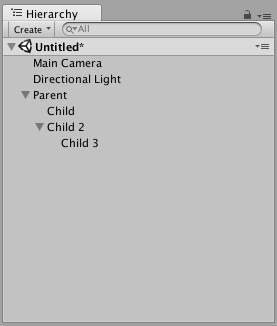
\includegraphics[width=0.25\textwidth]{figure/Hierarchy}
	\centering
	\caption{La finestra con la gerarchia.}
\end{figure}

\begin{flushleft}
	\underline{\textit{L'inspector}:}
	I progetti in Unity sono formati da molteplici GameObjects, i quali contengono scripts, suoni, meshes (modelli 3D), e altri elementi grafici come luci o canvas. La finestra denominata \textit{Inspector} permette la visualizzazione di suddette componenti sul GameObject selezionato. Le proprietà si possono vedere in dettaglio e modificare da questa finestra degli oggetti sulla scena o delle risorse non ancora istanziate nel mondo virtuale
\end{flushleft}

\begin{figure}[H]
	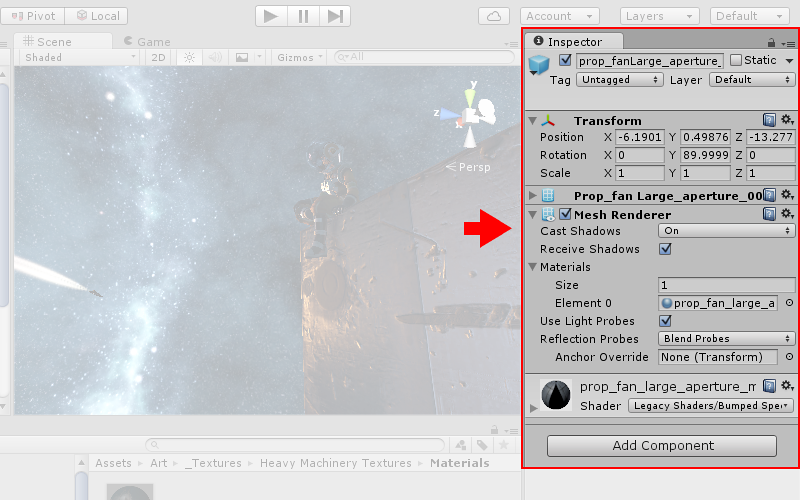
\includegraphics[width=0.45\textwidth]{figure/Inspector}
	\centering
	\caption{La finestra dell'Inspector.}
\end{figure}

\newpage

\begin{flushleft}
	\underline{\textit{La toolbar}:}
	La toolbar consiste in sette controlli base, ognuno dei quali connesso a parti dell'editor. I più importanti sono i bottoni di \textit{Play/Pause/Step}, che permettono l'inizio e la gestione della simulazione visibile nella finestra di gioco. 
	
\end{flushleft}

\begin{figure}[H]
	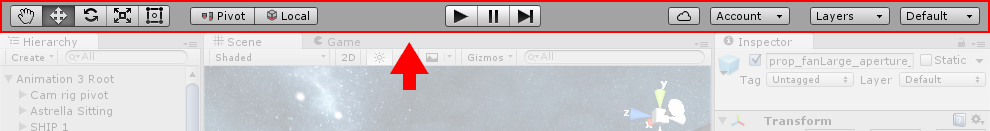
\includegraphics[width=0.55\textwidth]{figure/Toolbar}
	\centering
	\caption{La finestra contenente i controlli principali.}
\end{figure}

\begin{flushleft}
	\underline{\textit{Il gioco}:}
	In questa sezione viene renderizzata la telecamera principale presente nella scena, fornendo una rappresentazione di come verrà visualizzato il prodotto finale.
\end{flushleft}

\begin{figure}[H]
	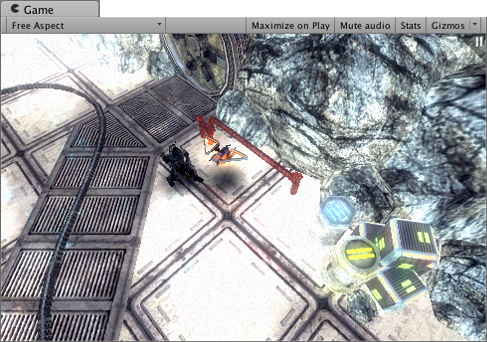
\includegraphics[width=0.55\textwidth]{figure/GameView}
	\centering
	\caption{La schermata che renderizza un'anteprima dell'applicazione finale.}
\end{figure}

\newpage
	

\subsection{Architettura Software di Unity}

In questa sottosezione verranno presentati brevemente le componenti software che stanno alla base del framework.

\subsubsection{Elementi Base}



\begin{flushleft}
	\underline{\textit{MonoBehaviour}:}
	MonoBehaviour è la classe base di Unity. Tutti i nuovi script sono sottoclassi di quest'ultima poiché MonoBehaviour fornisce i metodi che implementano il ciclo vitale di un'applicazione Unity.
	Se una classe deriva da MonoBehaviour allora potrà:
	 \begin{itemize}
	 	\item essere collegata agli oggetti Unity come una componente;
	 	\item fornire la possibilità di accedere alle sue variabili attraverso l'Inspector;
	 	\item supportare i metodi e gli eventi standard forniti da Unity come le funzioni Start(), OnGui(), Update() ecc.;
	 \end{itemize}
\end{flushleft}

\begin{flushleft}
\underline{\textit{GameObject}:}
GameObject è la classe principale per tutti gli oggetti esistenti in Unity. Ogni oggetto funge da contenitore che può avere al suo interno diversi elementi (componenti), le cui combinazioni possono conferire proprietà speciali. Ogni GameObject contiene di default la componente \textit{Transform} che ne definisce la posizione, la rotazione e la scala. Ogni GameObject presente nella scena può essere attivo o inattivo, in questo caso gli script collegati ad esso non saranno eseguiti ed eventuali mesh non saranno visualizzate.
\end{flushleft}

\begin{flushleft}
	\underline{\textit{Scripts}:}
Sono tutte le nuove classi che estendono MonoBehaviour. Quando uno script viene creato e connesso ad un oggetto ne diventa una componente. Quest'ultima verrà mostrata nell' Inspector assieme a tutte le variabili pubbliche contenute nella classe. Attraverso lo script è possibile accedere al GameObject e alle altre componenti ad esso connesse attraverso il metodo:
\begin{algorithmic}
	\STATE{public Component GetComponent<Type type>()}
\end{algorithmic}
ma non essendo un metodo molto veloce è consigliabile salvare nella cache la componente ritornata. 
\end{flushleft}

\newpage

\begin{flushleft}
	\underline{\textit{Prefab}:}
	Un prefab è un tipo di \textit{risorsa} che memorizza un GameObject e tutte le relative componenti e proprietà e funge da modello dal quale istanziare copie dell'oggetto nella scena. Ogni modifica effettuata sul prefab verrà riflessa sulle sue istanze sovrascrivendole. L'utilizzo di prefabs è vivamente consigliato poiché riduce i tempi di generazione e accesso degli oggetti nella memoria.
\end{flushleft}

\begin{flushleft}
	\underline{\textit{Resources}:}
	Unity non opera solamente con i prefabs ma anche con le \textit{resources} che possono essere texture, audio, video. La differenza con i prefabs è che una resource è sempre caricata nella scena cosi com'è e i cambiamenti apposti nell'editor non inficiano la resource iniziale, ma solo l'istanza modificata.
	Di default Unity crea resource di ogni asset presente nelle cartelle denominate "Resources" all'interno del progetto. Il contenuto di queste cartelle è sempre copiato nella build dell'applicazione.
\end{flushleft}

\begin{flushleft}
	\underline{\textit{Scene}:}
	Un'applicazione sviluppata con Unity non è altro che una composizione di scene, ognuna contenente gli ambienti e i menu. Si può pensare ad esse come a dei livelli, o più semplicemente delle schermate, che formano l'applicativo.
\end{flushleft}
 
 \begin{flushleft}
 	\underline{\textit{Packages}:}
 Unity permette l'esportazione di scene o oggetti in file, chiamati \textit{packages}. Il contenuto di questi ultimi può essere importato in qualsiasi progetto Unity. L'esportazione include tutte le dipendenze dei singoli oggetti, ovvero se si volesse esportare una scena, tutti i modelli, texture e altri asset al suo interno verrebbero automaticamente inclusi. Questa particolarità ha fatto si che Unity sviluppasse una grande community molto collaborativa.
 \end{flushleft}
 
 \newpage
\subsubsection{Ciclo di Vita}
In particolari momenti Unity chiama determinate funzioni, che ne compongono il ciclo vitale. Ogni script che estende MonoBehaviour può implementare o riscrivere questi metodi vitali. I più importanti sono descritte qui sotto.\\
\newline
I seguenti metodi sono chiamati all'inizio della scena, una volta per ogni oggetto nel frame:

\begin{flushleft}
\begin{algorithmic}
				\STATE{\textbf{Awake()}}
\end{algorithmic}
Il metodo Awake() viene chiamato quando l'istanza dello script viene caricata.
E' principalmente utilizzata per inizializzare variabili o stati prima che l'applicazione inizi ed è chiamata solamente una volta nel ciclo di vita dell'istanza. La sua chiamata viene effettuata solamente dopo che tutti gli oggetti nella scena sono stati inizializzati, perciò si può già comunicare con altri oggetti attraverso la funzione \begin{algorithmic}\STATE{public GameObject GameObject.Find()} \end{algorithmic} \vspace{0.4cm}
Awake() non viene chiamato negli oggetti inattivi presenti nella scena.
In particolare in C\# il metodo Awake() è utilizzato per l'inizializzazione invece di un costruttore, dato che lo stato serializzato dello script sarebbe ancora indefinito alla chiamata di quest'ultimo.
	
\end{flushleft}


\begin{flushleft}
	\begin{algorithmic}
		\STATE{\textbf{OnEnable()}}
	\end{algorithmic}
Questa funzione viene chiamata quando l'oggetto viene attivato. Utilizzata principalmente per la registrazione ad un evento.
	
\end{flushleft}


Le seguenti funzioni vengono invece chiamate sul primo frame dopo che lo script è stato attivato:
\begin{flushleft}
	\begin{algorithmic}
		\STATE{\textbf{Start()}}
	\end{algorithmic}
Viene eseguito Start() subito dopo la funzione Awake(), ma prima di ogni altra porzione di codice della classe. Come la funzione Awake() viene chiamata una sola volta nel ciclo vitale dello script.
\end{flushleft}


Al centro del ciclo vitale di Unity vi sono queste funzioni sottoelencate che vengono lanciate per l'intera vita dell'applicazione:

\begin{flushleft}
	\begin{algorithmic}
		\STATE{\textbf{FixedUpdate()}}
	\end{algorithmic}
	Questa funzione viene chiamata ad ogni \textit{fixed frame}, ovvero intervalli di tempo prestabiliti indipendenti dal frame rate dell'applicazione. Per questo motivo all'interno di questa funzione vengono gestite le componenti che computano la fisica della simulazione. Essendo le più dispendiose e le più importanti a livello visivo, esse così non vengono condizionate da eventuali rallentamenti nel gioco.
\end{flushleft}

\begin{flushleft}
	\begin{algorithmic}
		\STATE{\textbf{Update()}}
	\end{algorithmic}
	Il metodo Update() svolge un ruolo fondamentale nel ciclo vitale dell'applicazione ed è sicuramente il più usato. Viene eseguito una volta per ogni frame.  
\end{flushleft}

\begin{flushleft}
	\begin{algorithmic}
		\STATE{\textbf{LateUpdate()}}
	\end{algorithmic}
	Simile al metodo Update() ma viene eseguito subito dopo che tutti i processi di quest'ultimo sono terminati. 
\end{flushleft}


Infine i seguenti metodi sono utilizzati per gestire la disattivazione o morte di oggetti.

\begin{flushleft}
	\begin{algorithmic}
		\STATE{\textbf{OnDisable()}}
	\end{algorithmic}
	Chiamato quando un componente viene disattivato o reso inattivo, utilizzato maggiormente per cancellarsi dalle registrazioni degli eventi.
\end{flushleft}

\begin{flushleft}
	\begin{algorithmic}
		\STATE{\textbf{OnDestroy()}}
	\end{algorithmic}
	Chiamato nell'ultimo frame dell'esistenza dell'oggetto. Utilizzato per pulire la memoria da eventuali riferimenti.
\end{flushleft}

\begin{figure}[H]
	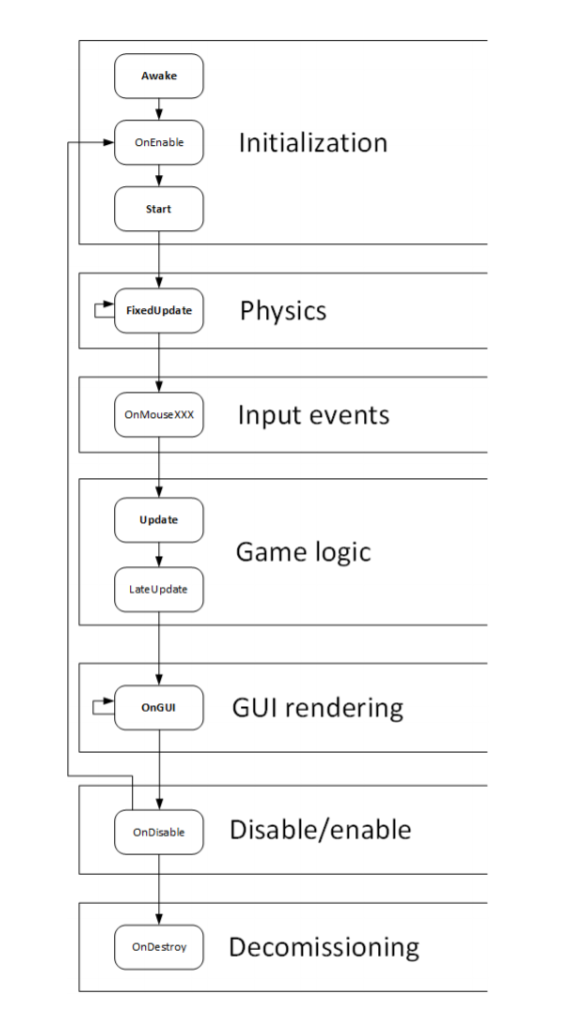
\includegraphics[width=0.55\textwidth]{figure/FunctionsScheme}
	\centering
	\caption{Questo schema mostra la sequenza delle chiamate alle principali funzioni di Unity.}
\end{figure}

\newpage
\section{Samsung Gear VR}

Il \textit{Samsung Gear VR} è un visore portatile  per la realtà virtuale sviluppado da \textit{Samsung Electronics} in collaborarzione con \textit{Oculus}, e prodotto da \textit{Samsung}. E' stato rilasciando nel Novembre 2015. Nell'utilizzo, un dispositivo compatibile (Galaxy Note 5, Galaxy S6/S6 Edge/S6 Edge+, Galaxy S7/S7 Edge, Galaxy S8/S8+ o Galaxy Note 8) funge da display e da processore, mentre l'unità Gear VR stessa funge da controller, contenente lenti focali e un'IMU. La connessione tra il visore ed il cellulare avviene tramite un connettore USB. Il Gear VR include anche un touchpad e bottoni fisici per la navigazione all'interno delle applicazione in caso non si possedesse un controller compatibile e un sensore di prossimità per determinare se l'utente lo sta indossando. La distanza focale in questo visore può essere calibrata attraverso una rotella posizionata nella parte superiore del prodotto, adattandosi all'utente. Le principali innovazioni apportate dal Gear Vr sono il raggiungimento di una latenza MTP(Motion to Photon) minore di 20ms e l'ottimizzazione dell'Hardware e del Kernel. \\

Unity forsnisce delle API di base per lo svilluppo su Gear VR senza l'utilizzo di plug-in esterni, che gestiscono la comunicazione tra una normale applicazione Android con il visore, trasformandola in un applicativo in realtà virtuale. Unity infatti gestisce automaticamente la renderizzazione delle camere presenti nella scena sul visore HMD (Head Mounted Display) generando le matrici di proiezione tenendo conto dei movimenti della testa e del campo visivo. E' invece compito dello sviluppatore preoccuparsi che il frame rate dell'applicazione non scenda sotto la frequenza di aggiornamento del display nel visore (60hz) nel caso del Gear VR o nascerebbero gli effetti collaterali precedentemente descritti. 
Per poter avviare applicazioni VR sui dispositivi Android compatibili va installato l'applicativo ufficiale Oculus Home che gestisce il lancio e l'esecuzione della nostra app.

 

 




